\documentclass[letterpaper,notitlepage,twoside]{article}

% Basic imports, increase margins...
\usepackage[margin=0.75in]{geometry}
\usepackage{amssymb}
\usepackage{amsmath}

% Finite State Machine stuff
\usepackage{pgf}
\usepackage{tikz}
\usetikzlibrary{arrows,automata}

% Format tables nicely
\usepackage[latin1]{inputenc}
\usepackage{array}
\usepackage{booktabs}
\setlength{\heavyrulewidth}{1.5pt}
\setlength{\abovetopsep}{4pt}

\usepackage{amsfonts} 
\usepackage{amssymb}
\usepackage{amsmath,amsthm}

\renewcommand{\implies}{\Rightarrow} % redefine command "implies"  
\renewcommand{\iff}{\Leftrightarrow} % double arrow
\newcommand{\maps}{\rightarrow} % define command "map" 
\newcommand{\union}{\cup}
\newcommand{\intersect}{\cap}
\newcommand{\N}{\mathbb{N}} % natural number 
\newcommand{\Q}{\mathbb{Q}} % rational number 
\newcommand{\R}{\mathbb{R}} % real number 
\newcommand{\Z}{\mathbb{Z}} % integers 
\newcommand\tab[1][1cm]{\hspace*{#1}} %\tab command

% Add more packages that you use here..

\title{CS 1510 Homework 2}
\author{Brian Falkenstein, Brian Knotten, Brett Schreiber}

\begin{document}
\maketitle

\section*{1}
Proof by counterexample: \\
Consider the following input: 
\begin{center}
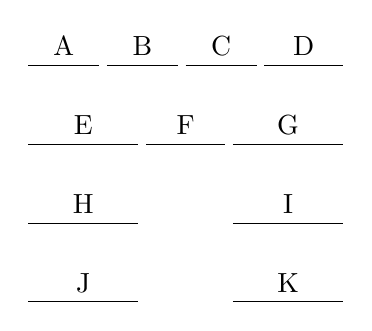
\begin{tikzpicture}
  \draw (0,3) -- node[above] {A} (0.9,3);
  \draw (1,3) -- node[above] {B} (1.9,3);
  \draw (2,3) -- node[above] {C} (2.9,3);
  \draw (3,3) -- node[above] {D} (4,3);
  \draw (0,2) -- node[above] {E} (1.4,2);
  \draw (1.5,2) -- node[above] {F} (2.5,2);
  \draw (2.6,2) -- node[above] {G} (4,2);
  \draw (0,1) -- node[above] {H} (1.4,1);
  \draw (2.6,1) -- node[above] {I} (4,1);
  \draw (0,0) -- node[above] {J} (1.4,0);
  \draw (2.6,0) -- node[above] {K} (4,0);
\end{tikzpicture}
\end{center}
The given Least Overlaps algorithm will clearly select $F$ as the first interval as it has the least number of overlaps (2) and $B$ and $C$ will be eliminated as the overlapping intervals. Next, the algorithm will arbitrarily select another interval as each of the remaining intervals overlaps 3 other intervals. Assuming $A$ is selected, $E$, $H$, and $J$ will be eliminated and the algorithm will proceed with selecting $D$, eliminating $G$, $I$, and $K$ and emptying $S$.\\
Therefore, the solution generated by the algorithm on the above input is $A$, $F$, $D$:
\begin{center}
\begin{tikzpicture}
 \draw (0,3) -- node[above] {A} (1,3);
 \draw (3,3) -- node[above] {D} (4,3);
 \draw (1.5,2) -- node[above] {F} (2.5,2);
\end{tikzpicture}
\end{center}
However, the obvious solution given the above input is $A$, $B$, $C$, $D$:
\begin{center}
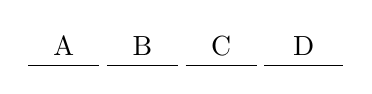
\begin{tikzpicture}
\draw (0,3) -- node[above] {A} (0.9,3);
  \draw (1,3) -- node[above] {B} (1.9,3);
  \draw (2,3) -- node[above] {C} (2.9,3);
  \draw (3,3) -- node[above] {D} (4,3);
\end{tikzpicture}
\end{center}
Therefore the algorithm does not solve the problem of generating a maximum cardinality subset of intervals given a set of intervals.

\section*{2}
\subsection*{a}
This algorithm $A$ does not find the optimal solution for the following instance $I$: For the first room, $A(I)$ chooses the interval that ends earliest, $A$. This eliminates $C$ and $D$ as candidates for the first room. The next room that ends earliest is $B$, which eliminates $E$, and now there are no intervals left, so the first room is full. $C$, $D$, and $E$ all overlap, so they must all have their own room. So $A(I)$ requires 4 rooms in its output: $\{A, B\}, \{C\}, \{D\}, \{E\}$. But a better solution exists using three rooms: $\{A, E\}, \{D, B\}, \{C\}$. So the algorithm $A$ is not correct in all instances.\
\\
\begin{center}
\begin{tikzpicture}
  \draw (0,3) -- node[above] {A} (2,3);
  \draw (5,3) -- node[above] {B} (6,3);
  \draw (1,2) -- node[above] {C} (7,2);
  \draw (1,1) -- node[above] {D} (4,1);
  \draw (3,0) -- node[above] {E} (7,0);
\end{tikzpicture}
\end{center}

\subsection*{b}
Assume the algorithm given, $A$, does not solve the interval coloring problem. Let $s$ be the maximum number of intervals that overlap at any point, and thus, the optimal output (minimum number of rooms after assigning all intervals). Then, $A$ will output a value larger than s for some input, and thus, $A$ does not solve the problem. We can conclude that in the case that $A$'s output is greater than $s$, this means that $A$ assigned a class to a new room when another room already had a space for it, as this would be the only case where $A$'s output could be greater than $s$. Because, in this algorithm, classes already placed are never altered / assigned to another room, this is a contradiction. The algorithm checks the set $R$ of rooms that already have a class scheduled in it, and places the class in the first room it finds that does not cause an overlap. Thus, the output of $A$ cannot be larger than s. 
~\\ \par
\end{document}
